\documentclass[twoside]{book}

% Packages required by doxygen
\usepackage{fixltx2e}
\usepackage{calc}
\usepackage{doxygen}
\usepackage[export]{adjustbox} % also loads graphicx
\usepackage{graphicx}
\usepackage[utf8]{inputenc}
\usepackage{makeidx}
\usepackage{multicol}
\usepackage{multirow}
\PassOptionsToPackage{warn}{textcomp}
\usepackage{textcomp}
\usepackage[nointegrals]{wasysym}
\usepackage[table]{xcolor}

% Font selection
\usepackage[T1]{fontenc}
\usepackage[scaled=.90]{helvet}
\usepackage{courier}
\usepackage{amssymb}
\usepackage{sectsty}
\renewcommand{\familydefault}{\sfdefault}
\allsectionsfont{%
  \fontseries{bc}\selectfont%
  \color{darkgray}%
}
\renewcommand{\DoxyLabelFont}{%
  \fontseries{bc}\selectfont%
  \color{darkgray}%
}
\newcommand{\+}{\discretionary{\mbox{\scriptsize$\hookleftarrow$}}{}{}}

% Page & text layout
\usepackage{geometry}
\geometry{%
  a4paper,%
  top=2.5cm,%
  bottom=2.5cm,%
  left=2.5cm,%
  right=2.5cm%
}
\tolerance=750
\hfuzz=15pt
\hbadness=750
\setlength{\emergencystretch}{15pt}
\setlength{\parindent}{0cm}
\setlength{\parskip}{3ex plus 2ex minus 2ex}
\makeatletter
\renewcommand{\paragraph}{%
  \@startsection{paragraph}{4}{0ex}{-1.0ex}{1.0ex}{%
    \normalfont\normalsize\bfseries\SS@parafont%
  }%
}
\renewcommand{\subparagraph}{%
  \@startsection{subparagraph}{5}{0ex}{-1.0ex}{1.0ex}{%
    \normalfont\normalsize\bfseries\SS@subparafont%
  }%
}
\makeatother

% Headers & footers
\usepackage{fancyhdr}
\pagestyle{fancyplain}
\fancyhead[LE]{\fancyplain{}{\bfseries\thepage}}
\fancyhead[CE]{\fancyplain{}{}}
\fancyhead[RE]{\fancyplain{}{\bfseries\leftmark}}
\fancyhead[LO]{\fancyplain{}{\bfseries\rightmark}}
\fancyhead[CO]{\fancyplain{}{}}
\fancyhead[RO]{\fancyplain{}{\bfseries\thepage}}
\fancyfoot[LE]{\fancyplain{}{}}
\fancyfoot[CE]{\fancyplain{}{}}
\fancyfoot[RE]{\fancyplain{}{\bfseries\scriptsize Generated by Doxygen }}
\fancyfoot[LO]{\fancyplain{}{\bfseries\scriptsize Generated by Doxygen }}
\fancyfoot[CO]{\fancyplain{}{}}
\fancyfoot[RO]{\fancyplain{}{}}
\renewcommand{\footrulewidth}{0.4pt}
\renewcommand{\chaptermark}[1]{%
  \markboth{#1}{}%
}
\renewcommand{\sectionmark}[1]{%
  \markright{\thesection\ #1}%
}

% Indices & bibliography
\usepackage{natbib}
\usepackage[titles]{tocloft}
\setcounter{tocdepth}{3}
\setcounter{secnumdepth}{5}
\makeindex

% Hyperlinks (required, but should be loaded last)
\usepackage{ifpdf}
\ifpdf
  \usepackage[pdftex,pagebackref=true]{hyperref}
\else
  \usepackage[ps2pdf,pagebackref=true]{hyperref}
\fi
\hypersetup{%
  colorlinks=true,%
  linkcolor=blue,%
  citecolor=blue,%
  unicode%
}

% Custom commands
\newcommand{\clearemptydoublepage}{%
  \newpage{\pagestyle{empty}\cleardoublepage}%
}

\usepackage{caption}
\captionsetup{labelsep=space,justification=centering,font={bf},singlelinecheck=off,skip=4pt,position=top}

%===== C O N T E N T S =====

\begin{document}

% Titlepage & ToC
\hypersetup{pageanchor=false,
             bookmarksnumbered=true,
             pdfencoding=unicode
            }
\pagenumbering{roman}
\begin{titlepage}
\vspace*{7cm}
\begin{center}%
{\Large My Project }\\
\vspace*{1cm}
{\large Generated by Doxygen 1.8.11}\\
\end{center}
\end{titlepage}
\clearemptydoublepage
\tableofcontents
\clearemptydoublepage
\pagenumbering{arabic}
\hypersetup{pageanchor=true}

%--- Begin generated contents ---
\chapter{Class Index}
\section{Class List}
Here are the classes, structs, unions and interfaces with brief descriptions\+:\begin{DoxyCompactList}
\item\contentsline{section}{\hyperlink{structnode}{node} }{\pageref{structnode}}{}
\item\contentsline{section}{\hyperlink{structnode1}{node1} }{\pageref{structnode1}}{}
\item\contentsline{section}{\hyperlink{structnode__info}{node\+\_\+info} }{\pageref{structnode__info}}{}
\end{DoxyCompactList}

\chapter{File Index}
\section{File List}
Here is a list of all files with brief descriptions\+:\begin{DoxyCompactList}
\item\contentsline{section}{\hyperlink{Lab1_8c}{Lab1.\+c} }{\pageref{Lab1_8c}}{}
\end{DoxyCompactList}

\chapter{Class Documentation}
\hypertarget{structPoint}{}\section{Point Struct Reference}
\label{structPoint}\index{Point@{Point}}
\subsection*{Public Attributes}
\begin{DoxyCompactItemize}
\item 
int \hyperlink{structPoint_a8c779e11e694b20e0946105a9f5de842}{x}
\item 
int \hyperlink{structPoint_a2e1b5fb2b2a83571f5c0bc0f66a73cf7}{y}
\end{DoxyCompactItemize}


\subsection{Member Data Documentation}
\index{Point@{Point}!x@{x}}
\index{x@{x}!Point@{Point}}
\subsubsection[{\texorpdfstring{x}{x}}]{\setlength{\rightskip}{0pt plus 5cm}int Point\+::x}\hypertarget{structPoint_a8c779e11e694b20e0946105a9f5de842}{}\label{structPoint_a8c779e11e694b20e0946105a9f5de842}
\index{Point@{Point}!y@{y}}
\index{y@{y}!Point@{Point}}
\subsubsection[{\texorpdfstring{y}{y}}]{\setlength{\rightskip}{0pt plus 5cm}int Point\+::y}\hypertarget{structPoint_a2e1b5fb2b2a83571f5c0bc0f66a73cf7}{}\label{structPoint_a2e1b5fb2b2a83571f5c0bc0f66a73cf7}


The documentation for this struct was generated from the following file\+:\begin{DoxyCompactItemize}
\item 
\hyperlink{ClosestPair_8cpp}{Closest\+Pair.\+cpp}\end{DoxyCompactItemize}

\chapter{File Documentation}
\hypertarget{ClosestPair_8cpp}{}\section{Closest\+Pair.\+cpp File Reference}
\label{ClosestPair_8cpp}\index{Closest\+Pair.\+cpp@{Closest\+Pair.\+cpp}}
{\ttfamily \#include $<$iostream$>$}\\*
{\ttfamily \#include $<$cfloat$>$}\\*
{\ttfamily \#include $<$cstdlib$>$}\\*
{\ttfamily \#include $<$cmath$>$}\\*
Include dependency graph for Closest\+Pair.\+cpp\+:
\nopagebreak
\begin{figure}[H]
\begin{center}
\leavevmode
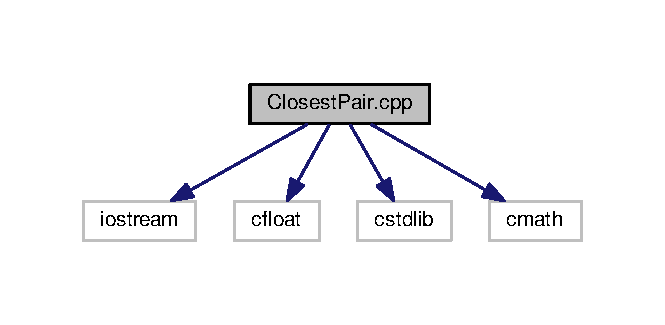
\includegraphics[width=319pt]{ClosestPair_8cpp__incl}
\end{center}
\end{figure}
\subsection*{Classes}
\begin{DoxyCompactItemize}
\item 
struct \hyperlink{structPoint}{Point}
\end{DoxyCompactItemize}
\subsection*{Functions}
\begin{DoxyCompactItemize}
\item 
int \hyperlink{ClosestPair_8cpp_a525d5d1c143aba1f71e6d705cb62760a}{compareX} (const void $\ast$a, const void $\ast$b)
\item 
int \hyperlink{ClosestPair_8cpp_a32bf76c194f25bd405c772667da96543}{compareY} (const void $\ast$a, const void $\ast$b)
\item 
float \hyperlink{ClosestPair_8cpp_a0b64710c8f93238fd1c94b878bbd182c}{dist} (\hyperlink{structPoint}{Point} p1, \hyperlink{structPoint}{Point} p2)
\item 
float \hyperlink{ClosestPair_8cpp_a146964a2a60bc7aad744097a83fbea22}{small\+\_\+dist} (\hyperlink{structPoint}{Point} P\mbox{[}$\,$\mbox{]}, int n)
\item 
float \hyperlink{ClosestPair_8cpp_a4cd5164639ea4c319b1fad38ab8e29bf}{strip\+Closest} (\hyperlink{structPoint}{Point} strip\mbox{[}$\,$\mbox{]}, int size, float d)
\item 
float \hyperlink{ClosestPair_8cpp_a1c20ec65873b12c96bee312d4b226eb3}{closest\+Util} (\hyperlink{structPoint}{Point} Px\mbox{[}$\,$\mbox{]}, \hyperlink{structPoint}{Point} Py\mbox{[}$\,$\mbox{]}, int n)
\item 
float \hyperlink{ClosestPair_8cpp_a763049a783bab63f349e117d2dde6adb}{closest} (\hyperlink{structPoint}{Point} P\mbox{[}$\,$\mbox{]}, int n)
\item 
int \hyperlink{ClosestPair_8cpp_ae66f6b31b5ad750f1fe042a706a4e3d4}{main} ()
\end{DoxyCompactItemize}


\subsection{Function Documentation}
\index{Closest\+Pair.\+cpp@{Closest\+Pair.\+cpp}!closest@{closest}}
\index{closest@{closest}!Closest\+Pair.\+cpp@{Closest\+Pair.\+cpp}}
\subsubsection[{\texorpdfstring{closest(\+Point P[], int n)}{closest(Point P[], int n)}}]{\setlength{\rightskip}{0pt plus 5cm}float closest (
\begin{DoxyParamCaption}
\item[{{\bf Point}}]{P\mbox{[}$\,$\mbox{]}, }
\item[{int}]{n}
\end{DoxyParamCaption}
)}\hypertarget{ClosestPair_8cpp_a763049a783bab63f349e117d2dde6adb}{}\label{ClosestPair_8cpp_a763049a783bab63f349e117d2dde6adb}

\begin{DoxyCode}
108 \{
109     \hyperlink{structPoint}{Point} Px[n];
110     \hyperlink{structPoint}{Point} Py[n];
111     \textcolor{keywordflow}{for} (\textcolor{keywordtype}{int} i = 0; i < n; i++)
112     \{
113         Px[i] = P[i];
114         Py[i] = P[i];
115     \}
116     qsort(Px, n, \textcolor{keyword}{sizeof}(\hyperlink{structPoint}{Point}), \hyperlink{ClosestPair_8cpp_a525d5d1c143aba1f71e6d705cb62760a}{compareX});
117     qsort(Py, n, \textcolor{keyword}{sizeof}(\hyperlink{structPoint}{Point}), \hyperlink{ClosestPair_8cpp_a32bf76c194f25bd405c772667da96543}{compareY});
118     \textcolor{keywordflow}{return} \hyperlink{ClosestPair_8cpp_a1c20ec65873b12c96bee312d4b226eb3}{closestUtil}(Px, Py, n);
119 \}
\end{DoxyCode}


Here is the call graph for this function\+:
\nopagebreak
\begin{figure}[H]
\begin{center}
\leavevmode
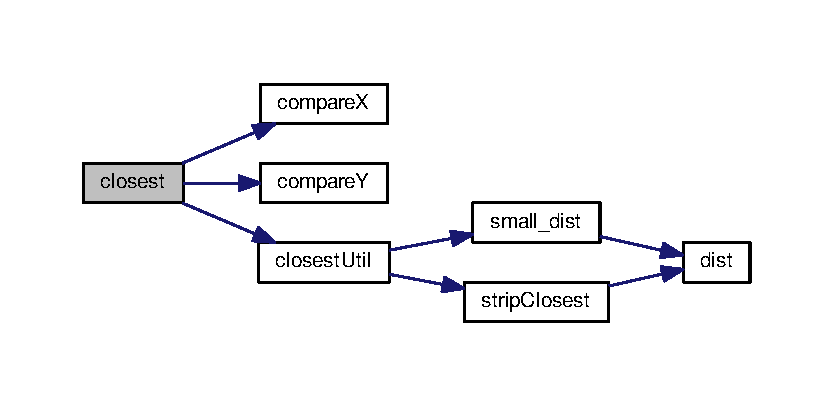
\includegraphics[width=350pt]{ClosestPair_8cpp_a763049a783bab63f349e117d2dde6adb_cgraph}
\end{center}
\end{figure}


\index{Closest\+Pair.\+cpp@{Closest\+Pair.\+cpp}!closest\+Util@{closest\+Util}}
\index{closest\+Util@{closest\+Util}!Closest\+Pair.\+cpp@{Closest\+Pair.\+cpp}}
\subsubsection[{\texorpdfstring{closest\+Util(\+Point Px[], Point Py[], int n)}{closestUtil(Point Px[], Point Py[], int n)}}]{\setlength{\rightskip}{0pt plus 5cm}float closest\+Util (
\begin{DoxyParamCaption}
\item[{{\bf Point}}]{Px\mbox{[}$\,$\mbox{]}, }
\item[{{\bf Point}}]{Py\mbox{[}$\,$\mbox{]}, }
\item[{int}]{n}
\end{DoxyParamCaption}
)}\hypertarget{ClosestPair_8cpp_a1c20ec65873b12c96bee312d4b226eb3}{}\label{ClosestPair_8cpp_a1c20ec65873b12c96bee312d4b226eb3}

\begin{DoxyCode}
77 \{
78     \textcolor{keywordflow}{if} (n <= 3)
79         \textcolor{keywordflow}{return} \hyperlink{ClosestPair_8cpp_a146964a2a60bc7aad744097a83fbea22}{small\_dist}(Px, n);
80     \textcolor{keywordtype}{int} mid = n / 2;
81     \hyperlink{structPoint}{Point} midPoint = Px[mid];
82     \hyperlink{structPoint}{Point} Pyl[mid + 1];
83     \hyperlink{structPoint}{Point} Pyr[n - mid - 1];
84     \textcolor{keywordtype}{int} li = 0, ri = 0;
85     \textcolor{keywordflow}{for} (\textcolor{keywordtype}{int} i = 0; i < n; i++)
86     \{
87         \textcolor{keywordflow}{if} (Py[i].x <= midPoint.\hyperlink{structPoint_a8c779e11e694b20e0946105a9f5de842}{x})
88             Pyl[li++] = Py[i];
89         \textcolor{keywordflow}{else}
90             Pyr[ri++] = Py[i];
91     \}
92     \textcolor{keywordtype}{float} dl = \hyperlink{ClosestPair_8cpp_a1c20ec65873b12c96bee312d4b226eb3}{closestUtil}(Px, Pyl, mid);
93     \textcolor{keywordtype}{float} dr = \hyperlink{ClosestPair_8cpp_a1c20ec65873b12c96bee312d4b226eb3}{closestUtil}(Px + mid, Pyr, n-mid);
94     \textcolor{keywordtype}{float} d = min(dl, dr);
95     \hyperlink{structPoint}{Point} strip[n];
96     \textcolor{keywordtype}{int} j = 0;
97     \textcolor{keywordflow}{for} (\textcolor{keywordtype}{int} i = 0; i < n; i++)
98     \{
99         \textcolor{keywordflow}{if} (abs(Py[i].x - midPoint.\hyperlink{structPoint_a8c779e11e694b20e0946105a9f5de842}{x}) < d)
100             strip[j] = Py[i], j++;
101     \}
102     \textcolor{keywordflow}{return} min(d, \hyperlink{ClosestPair_8cpp_a4cd5164639ea4c319b1fad38ab8e29bf}{stripClosest}(strip, j, d));
103 \}
\end{DoxyCode}


Here is the call graph for this function\+:
\nopagebreak
\begin{figure}[H]
\begin{center}
\leavevmode
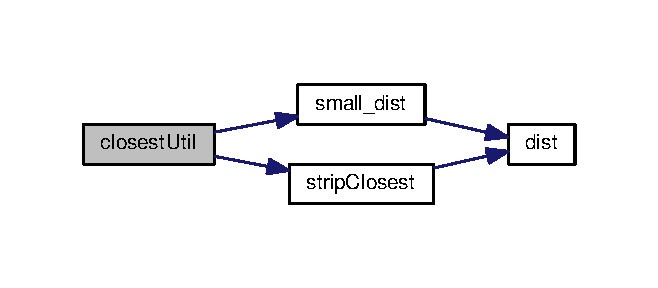
\includegraphics[width=316pt]{ClosestPair_8cpp_a1c20ec65873b12c96bee312d4b226eb3_cgraph}
\end{center}
\end{figure}


\index{Closest\+Pair.\+cpp@{Closest\+Pair.\+cpp}!compareX@{compareX}}
\index{compareX@{compareX}!Closest\+Pair.\+cpp@{Closest\+Pair.\+cpp}}
\subsubsection[{\texorpdfstring{compare\+X(const void $\ast$a, const void $\ast$b)}{compareX(const void *a, const void *b)}}]{\setlength{\rightskip}{0pt plus 5cm}int compareX (
\begin{DoxyParamCaption}
\item[{const void $\ast$}]{a, }
\item[{const void $\ast$}]{b}
\end{DoxyParamCaption}
)}\hypertarget{ClosestPair_8cpp_a525d5d1c143aba1f71e6d705cb62760a}{}\label{ClosestPair_8cpp_a525d5d1c143aba1f71e6d705cb62760a}

\begin{DoxyCode}
22 \{
23     \hyperlink{structPoint}{Point} *p1 = (\hyperlink{structPoint}{Point} *)a, *p2 = (\hyperlink{structPoint}{Point} *)b;
24     \textcolor{keywordflow}{return} (p1->\hyperlink{structPoint_a8c779e11e694b20e0946105a9f5de842}{x} - p2->x);
25 \}
\end{DoxyCode}
\index{Closest\+Pair.\+cpp@{Closest\+Pair.\+cpp}!compareY@{compareY}}
\index{compareY@{compareY}!Closest\+Pair.\+cpp@{Closest\+Pair.\+cpp}}
\subsubsection[{\texorpdfstring{compare\+Y(const void $\ast$a, const void $\ast$b)}{compareY(const void *a, const void *b)}}]{\setlength{\rightskip}{0pt plus 5cm}int compareY (
\begin{DoxyParamCaption}
\item[{const void $\ast$}]{a, }
\item[{const void $\ast$}]{b}
\end{DoxyParamCaption}
)}\hypertarget{ClosestPair_8cpp_a32bf76c194f25bd405c772667da96543}{}\label{ClosestPair_8cpp_a32bf76c194f25bd405c772667da96543}

\begin{DoxyCode}
30 \{
31     \hyperlink{structPoint}{Point} *p1 = (\hyperlink{structPoint}{Point} *)a, *p2 = (\hyperlink{structPoint}{Point} *)b;
32     \textcolor{keywordflow}{return} (p1->\hyperlink{structPoint_a2e1b5fb2b2a83571f5c0bc0f66a73cf7}{y} - p2->y);
33 \}
\end{DoxyCode}
\index{Closest\+Pair.\+cpp@{Closest\+Pair.\+cpp}!dist@{dist}}
\index{dist@{dist}!Closest\+Pair.\+cpp@{Closest\+Pair.\+cpp}}
\subsubsection[{\texorpdfstring{dist(\+Point p1, Point p2)}{dist(Point p1, Point p2)}}]{\setlength{\rightskip}{0pt plus 5cm}float dist (
\begin{DoxyParamCaption}
\item[{{\bf Point}}]{p1, }
\item[{{\bf Point}}]{p2}
\end{DoxyParamCaption}
)}\hypertarget{ClosestPair_8cpp_a0b64710c8f93238fd1c94b878bbd182c}{}\label{ClosestPair_8cpp_a0b64710c8f93238fd1c94b878bbd182c}

\begin{DoxyCode}
38 \{
39     \textcolor{keywordflow}{return} sqrt((p1.\hyperlink{structPoint_a8c779e11e694b20e0946105a9f5de842}{x} - p2.\hyperlink{structPoint_a8c779e11e694b20e0946105a9f5de842}{x}) * (p1.\hyperlink{structPoint_a8c779e11e694b20e0946105a9f5de842}{x} - p2.\hyperlink{structPoint_a8c779e11e694b20e0946105a9f5de842}{x}) + (p1.\hyperlink{structPoint_a2e1b5fb2b2a83571f5c0bc0f66a73cf7}{y} - p2.\hyperlink{structPoint_a2e1b5fb2b2a83571f5c0bc0f66a73cf7}{y}) * (p1.\hyperlink{structPoint_a2e1b5fb2b2a83571f5c0bc0f66a73cf7}{y} - p2.
      \hyperlink{structPoint_a2e1b5fb2b2a83571f5c0bc0f66a73cf7}{y}));
40 \}
\end{DoxyCode}
\index{Closest\+Pair.\+cpp@{Closest\+Pair.\+cpp}!main@{main}}
\index{main@{main}!Closest\+Pair.\+cpp@{Closest\+Pair.\+cpp}}
\subsubsection[{\texorpdfstring{main()}{main()}}]{\setlength{\rightskip}{0pt plus 5cm}int main (
\begin{DoxyParamCaption}
{}
\end{DoxyParamCaption}
)}\hypertarget{ClosestPair_8cpp_ae66f6b31b5ad750f1fe042a706a4e3d4}{}\label{ClosestPair_8cpp_ae66f6b31b5ad750f1fe042a706a4e3d4}

\begin{DoxyCode}
125 \{
126     \hyperlink{structPoint}{Point} P[] = \{\{2, 3\}, \{12, 30\}, \{40, 50\}, \{5, 1\}, \{12, 10\}, \{3, 4\}\};
127     \textcolor{keywordtype}{int} n = \textcolor{keyword}{sizeof}(P) / \textcolor{keyword}{sizeof}(P[0]);
128     cout << \textcolor{stringliteral}{"The smallest distance is "} << \hyperlink{ClosestPair_8cpp_a763049a783bab63f349e117d2dde6adb}{closest}(P, n);
129     \textcolor{keywordflow}{return} 0;
130 \}\end{DoxyCode}


Here is the call graph for this function\+:
\nopagebreak
\begin{figure}[H]
\begin{center}
\leavevmode
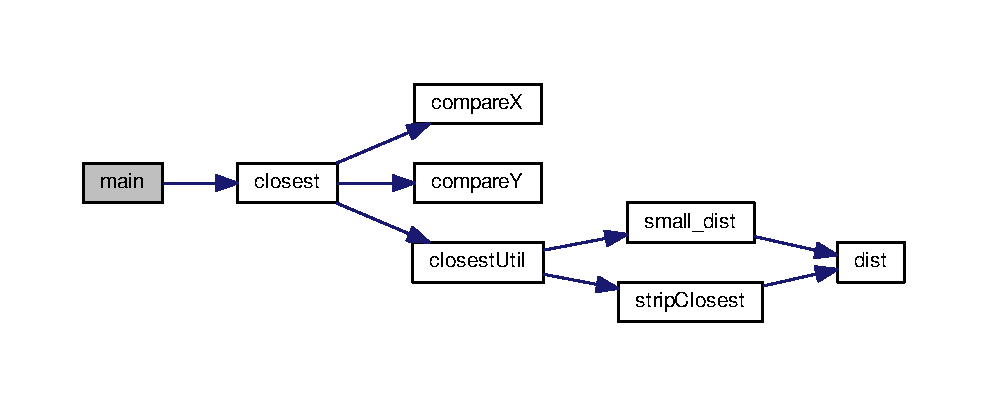
\includegraphics[width=350pt]{ClosestPair_8cpp_ae66f6b31b5ad750f1fe042a706a4e3d4_cgraph}
\end{center}
\end{figure}


\index{Closest\+Pair.\+cpp@{Closest\+Pair.\+cpp}!small\+\_\+dist@{small\+\_\+dist}}
\index{small\+\_\+dist@{small\+\_\+dist}!Closest\+Pair.\+cpp@{Closest\+Pair.\+cpp}}
\subsubsection[{\texorpdfstring{small\+\_\+dist(\+Point P[], int n)}{small_dist(Point P[], int n)}}]{\setlength{\rightskip}{0pt plus 5cm}float small\+\_\+dist (
\begin{DoxyParamCaption}
\item[{{\bf Point}}]{P\mbox{[}$\,$\mbox{]}, }
\item[{int}]{n}
\end{DoxyParamCaption}
)}\hypertarget{ClosestPair_8cpp_a146964a2a60bc7aad744097a83fbea22}{}\label{ClosestPair_8cpp_a146964a2a60bc7aad744097a83fbea22}

\begin{DoxyCode}
45 \{
46     \textcolor{keywordtype}{float} min = FLT\_MAX;
47     \textcolor{keywordflow}{for} (\textcolor{keywordtype}{int} i = 0; i < n; ++i)
48     \{
49         \textcolor{keywordflow}{for} (\textcolor{keywordtype}{int} j = i + 1; j < n; ++j)
50         \{
51             \textcolor{keywordflow}{if} (\hyperlink{ClosestPair_8cpp_a0b64710c8f93238fd1c94b878bbd182c}{dist}(P[i], P[j]) < min)
52                 min = \hyperlink{ClosestPair_8cpp_a0b64710c8f93238fd1c94b878bbd182c}{dist}(P[i], P[j]);
53         \}
54     \}
55     \textcolor{keywordflow}{return} min;
56 \}
\end{DoxyCode}


Here is the call graph for this function\+:
\nopagebreak
\begin{figure}[H]
\begin{center}
\leavevmode
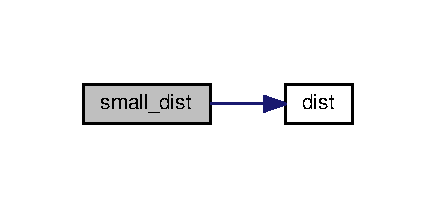
\includegraphics[width=209pt]{ClosestPair_8cpp_a146964a2a60bc7aad744097a83fbea22_cgraph}
\end{center}
\end{figure}


\index{Closest\+Pair.\+cpp@{Closest\+Pair.\+cpp}!strip\+Closest@{strip\+Closest}}
\index{strip\+Closest@{strip\+Closest}!Closest\+Pair.\+cpp@{Closest\+Pair.\+cpp}}
\subsubsection[{\texorpdfstring{strip\+Closest(\+Point strip[], int size, float d)}{stripClosest(Point strip[], int size, float d)}}]{\setlength{\rightskip}{0pt plus 5cm}float strip\+Closest (
\begin{DoxyParamCaption}
\item[{{\bf Point}}]{strip\mbox{[}$\,$\mbox{]}, }
\item[{int}]{size, }
\item[{float}]{d}
\end{DoxyParamCaption}
)}\hypertarget{ClosestPair_8cpp_a4cd5164639ea4c319b1fad38ab8e29bf}{}\label{ClosestPair_8cpp_a4cd5164639ea4c319b1fad38ab8e29bf}

\begin{DoxyCode}
61 \{
62     \textcolor{keywordtype}{float} min = d;
63     \textcolor{keywordflow}{for} (\textcolor{keywordtype}{int} i = 0; i < size; ++i)
64     \{
65         \textcolor{keywordflow}{for} (\textcolor{keywordtype}{int} j = i + 1; j < size && (strip[j].\hyperlink{structPoint_a2e1b5fb2b2a83571f5c0bc0f66a73cf7}{y} - strip[i].\hyperlink{structPoint_a2e1b5fb2b2a83571f5c0bc0f66a73cf7}{y}) < min; ++j)
66         \{
67             \textcolor{keywordflow}{if} (\hyperlink{ClosestPair_8cpp_a0b64710c8f93238fd1c94b878bbd182c}{dist}(strip[i],strip[j]) < min)
68                 min = \hyperlink{ClosestPair_8cpp_a0b64710c8f93238fd1c94b878bbd182c}{dist}(strip[i], strip[j]);
69         \}
70     \}
71     \textcolor{keywordflow}{return} min;
72 \}
\end{DoxyCode}


Here is the call graph for this function\+:
\nopagebreak
\begin{figure}[H]
\begin{center}
\leavevmode
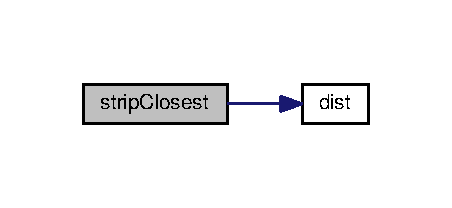
\includegraphics[width=217pt]{ClosestPair_8cpp_a4cd5164639ea4c319b1fad38ab8e29bf_cgraph}
\end{center}
\end{figure}



%--- End generated contents ---

% Index
\backmatter
\newpage
\phantomsection
\clearemptydoublepage
\addcontentsline{toc}{chapter}{Index}
\printindex

\end{document}
